\section{Graded Assignment 2}\label{sec:graded_assignment_2}

% A full answer and result analysis is expected for task 3 and 4. For task 3 you should include a plot of the different states over time as well as the error states for your choice of parameters, in addition to NEES and NIS over time for the same set of parameters. In task 4 the same plots are expected, of course excluding anything that needs the ground truth. For both tasks it should be made clear why the parameters were chosen in terms of error metrics, consistency and overall result. Answers and analysis should connect theory and results to the real world, and show your understanding for the problem and solution. Try to connect the reuslts on the simulated data to the results of the real data where it is possible. 

An error-state Kalman filter was implemented in MATLAB. For the relevant theory behind the implementation, see \cite{Sola} and \cite{Edmund}.

\begin{figure}[!htb]
    \centering
    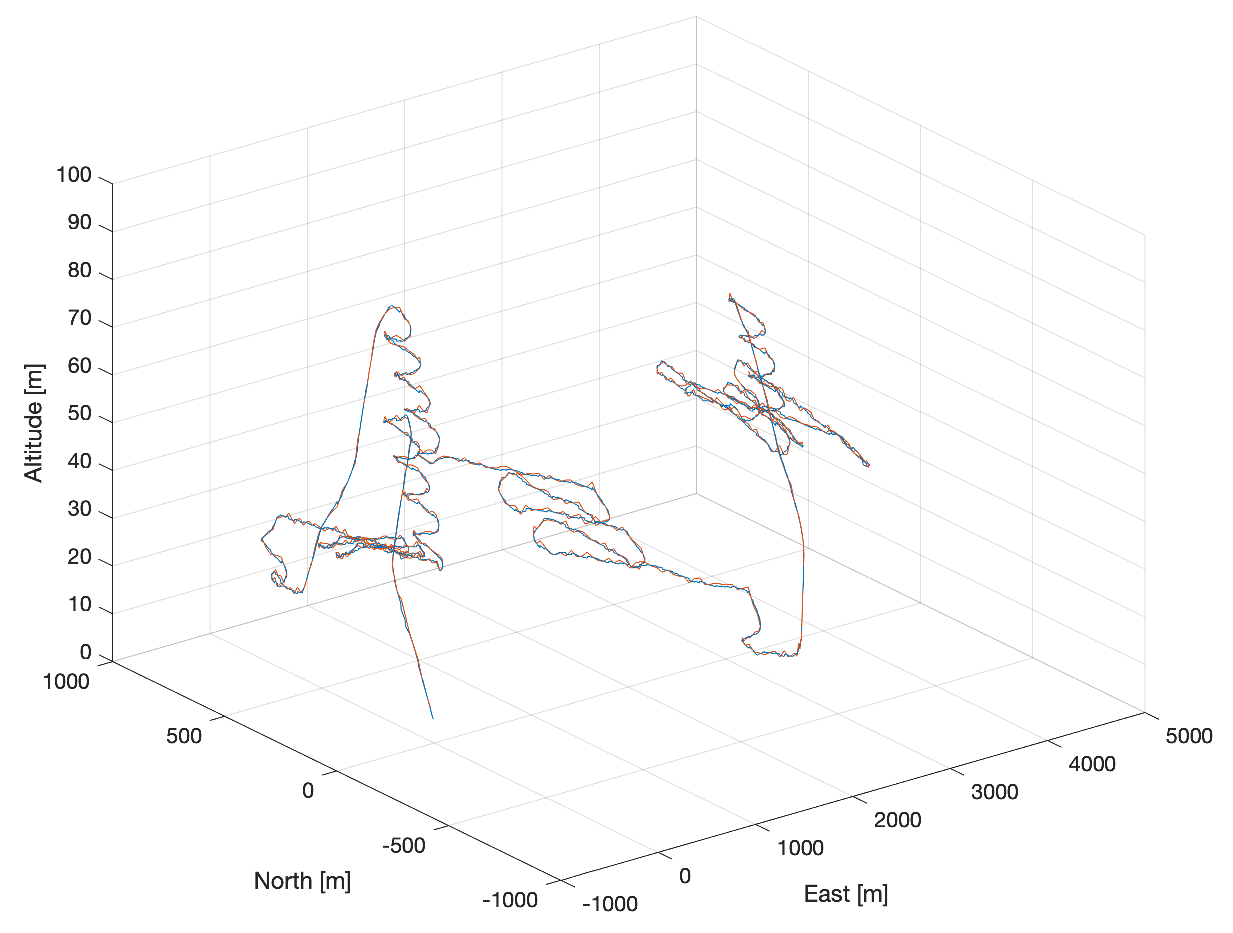
\includegraphics{figures/ga_2/sim_trajectory.eps}
    \caption{}
    \label{}
\end{figure}